\section{Modeling of risk transfer mechanisms}

\subsection{Risk Transfer structure}

Sometime, the financial position of a legal entity is inadequate towards its risk profile. The company can be under-capitalized compared to the level of risks it underwrote, which is dangerous for shareholders and policyholders. On the other end, a company can be over-capitalized. This can be the case if the legal entity is newly opened and the regulator required a very strong capitalization to grant the reinsurance license. This case is not optimal for shareholders, whose return on capital is sub-optimal. Such cases lead to the desire of finding means to re-balance the risk profile and the financial position of companies. 

To that end, two means are available. The first mean is capital transfer (called capital injection) from one company to another (within the group). In section \ref{sec:OWNERSHIP}, the ownership structure of a reinsurance group was presented as a first type of relation between companies. This structure is important to study the flow of dividends from subsidiaries to the mother company. But this ownership structure also constrains the capacities of capital transfers from one company to another. Transferring capital from one company to another, operation called "Capital injection", is a complex legal operation that cannot be performed easily and quickly.
Instead of transferring capital between companies, another way is to transfer risks from one company to another. This kind of risk transfer is the core of the insurer and re-insurer skill. In the context of a risk transfer from one re-insurer to another, the agreement is called a retrocession agreement. The use of retrocession is much easier than capital injection as it is exactly the product sold by a re-insurer. Moreover, it can be used within a group (internal retrocession) or with other companies (external retrocession). With internal retrocession, profits stay inside the group but the risk too : it is just transferred from one legal entity to another.

An example of risk transfer structure through internal retrocession is presented in Figure \ref{fig:GROUP_STRUCTURE}. Risk transfer link are the red arrows.

A reinsurance company is generally re-insured through external retrocessions against extreme losses on several of its lines of businesses. It is a way to spread the risk through the entire industry and limit the probability of default of re-insurers. Each company is free to choose its own external retrocession program, but the more it retrocede risk, the more its profitability is reduced. Therefore, a re-insurer must find the good balance by according its retrocession program with its risk appetite.

To understand the concept of retrocession, let's assume that a legal entity have a retrocession program with an external reinsurance company. This retrocession program state that $\frac{1}{10}$ of all losses will be transferred from the company to the retrocessionaire. If the company bear a "gross" loss of \$ 100 M, \$ 10 M will be paid by the retrocessionaire and the "net" loss of the company is \$ 90 M. The "gross" loss is the initial loss that the underwriting company must pay to its policyholders. After deduction of the contribution of the retrocessionaires, the final loss bore by the company is called the "net" loss. The difference between the "gross" loss and the "net loss" is the part of the loss that is paid by the retrocessionaires (and can be called "the retrocession").

TODO : METTRE FIGURE

These terms can be confusing because there is no word difference between an external retrocession and an internal retrocession. A net loss can be after external retrocession, internal retrocession, or after both external and internal retrocession.


\subsection{Proportional and Non proportional reinsurance}

Reinsurance treaties can be proportional or non proportional. An example of proportional treaty is the quota-share (QS) treaty. A quota-share treaty consists in the transfer of an agreed share of risk $\alpha$ from the ceding company (the cedent) to a retrocessionaire. As the share $\alpha$ of the risk is ceded, a share $\alpha$ of premium are also transfered to the retrocessionaire (in practice a commission is paid back by the retrocessionaire to compensate the reinsurer costs) (see \ref{fig:TYPE_RETROCESSION}). 

Two examples of non proportional treaties are provided in \ref{fig:TYPE_RETROCESSION}. The first type of non proportional treaty is the "Excess of Loss" treaty. In this type of treaty, the retrocessionaire must pay losses exceeding a certain limit called "Priority" (or "Deductible") up to a limit called the "Limit" (or "Coverage"). If the Limit is infinite, the treaty is considered as a "Stop Loss".

Treaties can be associated to a risk or an event. In the case of a risk trigger, the treaty is activated for every risk occurring. For example, if a treaty is protecting a portfolio of people with death insurance, the treaty will be activated each time a person dies. To activate an event treaty, the must be at least two risk occurring simultaneously. This type of treaty is generally used to protect against natural catastrophes or event where aggregation of risk of very likely.


\begin{figure}[h!]
  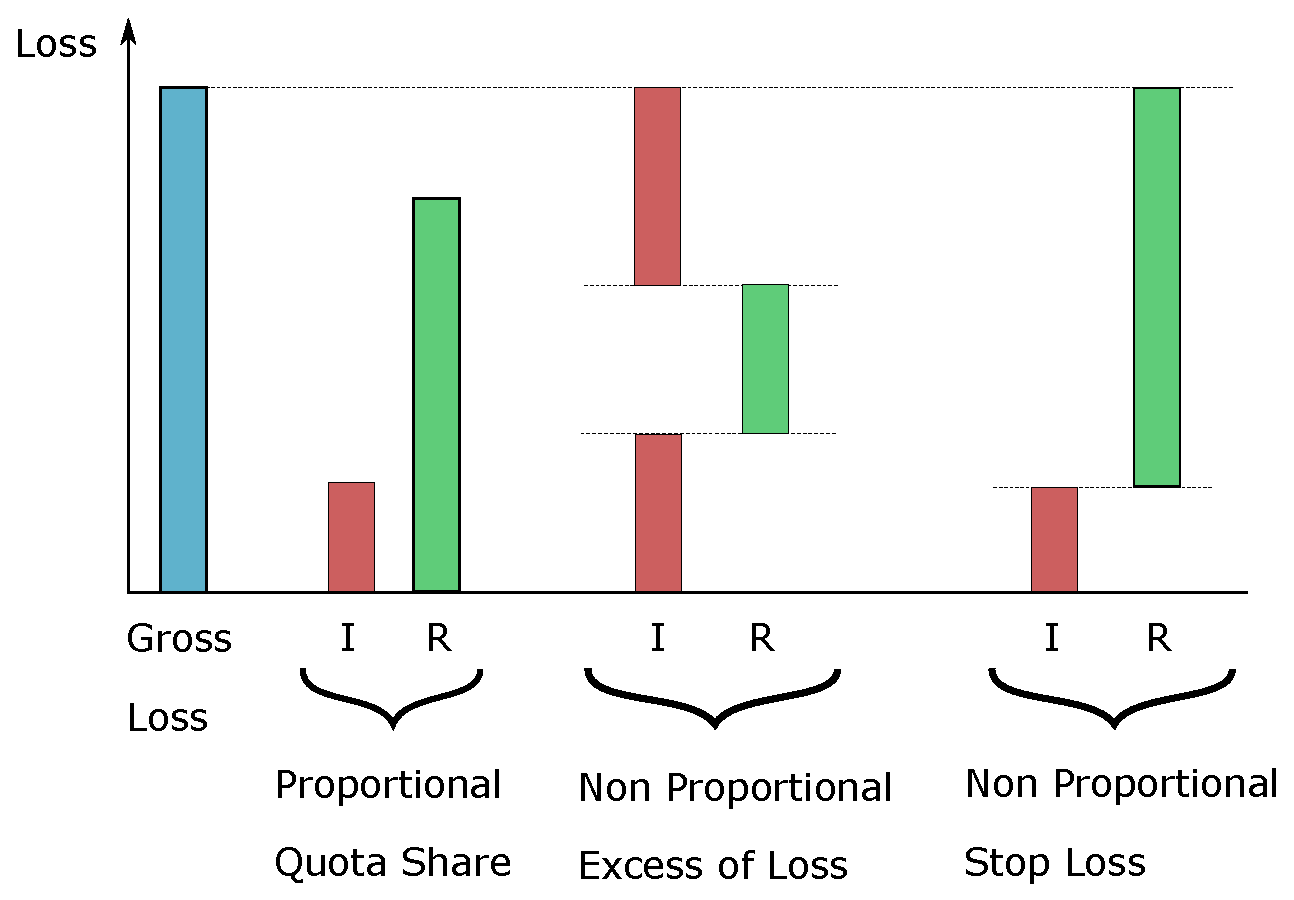
\includegraphics[width=\linewidth]{images/part1/type_retrocession.eps}
  \caption{Several type of retrocession agreement. (blue) Gross loss of the insurer, (red) share of the loss attributable to the insurer, (green) loss attributable to the reinsurer (or retrocessionaire). The cession share of the quota share agreement is 80\%.}
  \label{fig:TYPE_RETROCESSION}
\end{figure}


\subsection{Modeling of external retrocession}


TODO : COMMENT EST GERE DANS UNE BOITE ?


\subsection{Modeling internal Retrocession}

Before any shock (loss) applied on legal entities, losses are null, meaning that :

\begin{equation}
    L = (0)_{i \in [1, N]}
\end{equation}

After a shock is applied, each entity suffers a loss of $L$:

\begin{equation}
    L^0 = (L_i^0)_{i \in [1, N]}
\end{equation}

After external retrocession is applied, the loss vector is denoted:

\begin{equation}
    L = (L_i)_{i \in [1, N]}
\end{equation}


However, it is assumed that internal retrocession agreements exist between entities. The loss vector after use of these retrocessions is denoted $L^U$, the superscript $U$ meaning "updated":

\begin{equation}
    L^U = (L_i^U)_{i \in [1, N]}
\end{equation}


We propose to model the retrocession agreement between two legal entities by a function $r_{i \gets j}$ taking the full loss vector $L$ as an input and outputting the amount of loss transferred from entity $j$ to entity $i$. $i$ and $j$ belong to $[1, N]$

\begin{equation}
    r_{i \gets j} : L \in \R^N \to \R
\end{equation}

For simplicity, it is assumed that the values of $r_{i \gets j}$ are always \textbf{positive}.

For instance, a proportional retrocession from entity $A$ to entity $B$ is written :

\begin{equation}
    r_{B \gets A}^{proportional}(L)  = \alpha_{B \gets A} L_A
\end{equation}

with $\alpha_{ B \gets A} \in [0, 1]$ and $L_A$ the loss of entity $A$.

While a proportional retrocession from entity $B$ to entity $A$ is written :

\begin{equation}
    r_{A \gets B}^{proportional}(L)  = \alpha_{A \gets B} L_A
\end{equation}

An excess of loss agreement from A to B without deductible and limited at $M_{BA}$ is written:

\begin{equation}
    r_{B \gets A}^{excess loss}(L)  =  min(L_B, M_{BA})
\end{equation}


Considering this definition of retrocession loss transfer, how to computer $L^U$ from $L^0$ and the collection of $(r_{i \gets j})_{(i, j)}$?

We define the operator $R[]$ by the following relation :

\begin{equation}
    L^U = R[L]
\end{equation}

$L$ and $L^U$ are vector belonging to $\R^N$ and the operator $R[]$ applies the following operation :

\begin{equation}
\label{def_R}
    R[L] = \left( \sum_j r_{i \gets j}(L) \right)_{(i \in [1, N])}
\end{equation}

The brackets $[]$ of $R[]$ denote the sum over the columns of $R$, while $R$ is a matrix of functions, containing the retrocession functions (incomplete representation at this stage of the model presentation) :

\begin{equation}
R = 
\begin{pmatrix}
? & r_{1 \gets 2} & r_{1 \gets 2} & ... & r_{1 \gets N}\\
r_{2 \gets 1} & ? & r_{2 \gets 3} & ... & r_{2 \gets N}\\
\vdots & \vdots & \vdots & \vdots & \vdots\\
r_{N \gets 1} & r_{N \gets 3} & ... & r_{N \gets (N-1)} & ?
\end{pmatrix}
\end{equation}

The matrix $R$ is called the "Retrocession Matrix" and is a N by N square matrix. Each line of the matrix represent a loss receiving entity and each column a loss giving entity.

Expression \ref{def_R} means that the ith element of the updated loss $L^U$ is the sum of all losses given by other entities. For $i \neq j$, the retrocession function $r_{i \gets j}$ was defined before. The case of $r_{i \gets i}$ is more complex.

If no retrocession agreement exist between the legal entities, then R must be the identify matrix, so that $L^U = L^0$.

Then the R matrix expression can be refined by writing :

\begin{equation}
R = 
\begin{pmatrix}
1 + ? & r_{1 \gets 2} & r_{1 \gets 2} & ... & r_{1 \gets N}\\
r_{2 \gets 1} & 1 + ? & r_{2 \gets 3} & ... & r_{2 \gets N}\\
\vdots & \vdots & \vdots & \vdots & \vdots\\
r_{N \gets 1} & r_{N \gets 3} & ... & r_{N \gets (N-1)} & 1 + ?
\end{pmatrix}
\end{equation}


Internal retrocession is a zero-sum game. This means that amount given by entity $ji$ to $j$, are received by $j$. This can be accounted by adding an additional terms to the diagonal elements of $R$:

\begin{equation}
R = 
\begin{pmatrix}
1 - (\sum_{i=2}^{N} r_{i \gets 1}) & r_{1 \gets 2} & r_{1 \gets 2} & ... & r_{1 \gets N}\\
r_{2 \gets 1} & 1 - (\sum_{i={1, 3, 4}}^{N} r_{i \gets 2}) & r_{2 \gets 3} & ... & r_{2 \gets N}\\
\vdots & \vdots & \vdots & \vdots & \vdots\\
r_{N \gets 1} & r_{N \gets 3} & ... & r_{N \gets (N-1)} & 1 - (\sum_{i={1}}^{N-1} r_{i \gets N})
\end{pmatrix}
\end{equation}

This additional terms compensate every given loss by its corresponding received one on the relevant entity.

According to these definitions, one can demonstrate that $\sum_i L_i^U = \sum_i L_i^0$, accounting for the fact that money is transferred between entities and no money flows in or out of the insurance group.



Here are sime exemple of Retrocession matrices in simple cases.

Lets assume two entities names 1 and 2, with crossed proportional retrocession agreements.

The loss vector is : 

\begin{equation}
L = 
\begin{pmatrix}
L_1 \\
L_2
\end{pmatrix}
\end{equation}

The R matrix is :
\begin{equation}
R = 
\begin{pmatrix}
1 - r_{2 \gets 1} & r_{1 \gets 2}\\
r_{2 \gets 1} & 1 - r_{1 \gets 2}
\end{pmatrix}
\end{equation}

with :
\begin{equation}
    r_{1 \gets 2} = \alpha_{1 \gets 2} L_2
\end{equation}

\begin{equation}
    r_{2 \gets 1} = \alpha_{2 \gets 1} L_1
\end{equation}

The full loss expression is then :

\begin{equation}
L^U = R[L] = 
\begin{pmatrix}
L_1 (1 - \alpha_{2 \gets 1}) + L_2 \alpha_{1 \gets 2} \\
L_1 \alpha_{2 \gets 1} + L_2 (1 - \alpha_{1 \gets 2})
\end{pmatrix}
\end{equation}

This matrix make sense: entity 1's updated loss $L_1^U$ is the loss $L_1$ at time 0 minus the loss given to 2 plus the loss received from 2.

In the case of excess of loss without deductible whose maximum amount are $M_{1 \gets 2}$ and $M_{2 \gets 1}$:

\begin{equation}
    r_{1 \gets 2} = min(L_2, M_{1 \gets 2})
\end{equation}
\begin{equation}
    r_{2 \gets 1} = min(L_1, M_{2 \gets 1})
\end{equation}

The full loss expression is :

\begin{equation}
L^U = R[L] = 
\begin{pmatrix}
L_1 - min(L_1, M_{2 \gets 1}) + min(L_2, M_{1 \gets 2} \\
L_2 + min(L_1, M_{2 \gets 1}) - min(L_2, M_{1 \gets 2}
\end{pmatrix}
\end{equation}

The flexibility of on the definition of $r_{i \gets j}$ allows for function composition, for instance a quota share followed by and excess of loss.

Moreover, in this model, all retrocession operation are realized at the exact same time. Amount are all "transferred" at the same moment and received funds are not cyclically taken into account. Cases of multistep retrocessions can be taken into account by compounding the Retrocession matrix with another one representing the next step of retrocessions. A single complex Retrocession matrix is obtained by compounding the several retrocessions steps.




Cp = Ci - R * L


Hypothèse : RC = RCi
SR = Cp / RCi
SR =  (Ci - R * L) / RCi
SR = SRi - R * (L / RCi)
deltaSR = R * ( L / RCi )

objectif : minimser deltaSR
